\chapter{Endgames: Perfect Situation in~Perfect-Information Games}

For many games, solving their late stages (so-called \emph{endgames}) can be done in~an~online way.
In other words, we are often able to postpone the computation of~the endgame strategy until the endgame itself is reached in~the play.

This is especially the case of~perfect-information games such as chess or Go, where the endgame technique has been used for long time.
In these domains, online endgame solving has~significant importance, as it substantially improves the playing quality of~agents.

\section{Chess Endgames}

\subsection{What are Endgames in Chess?}

The notion of~``endgame'' has no strict definition and greatly differs by various authors.
The common sense says it begins with only few pieces left.
Here are some examples of~various approaches to defining endgames:
\begin{itemize}
  \item
    positions in which each player has less than thirteen points in material (not counting the king)
    (\cite[pp.~7--8]{Speelman1981endgame})
    
  \item
    positions in which the king can be used actively (but there are some famous exceptions to that)
    (\cite[pp.~7--8]{Speelman1981endgame})
    
  \item
    positions having four or fewer pieces other than kings and pawns
    (\cite[p.~5]{Minev2004practical})
    
  \item
    positions without queens
    (\cite{Fine1952middle}),
    
  \item
    positions when each player has less than a queen plus rook in material
    
  \item
    positions when the player who is about to move can force a~win or a~draw against any variation of~moves
    (\cite{Portisch1981six})

  \item 
    positions with these three characteristics~(\cite{Alburt1999just}):

    \begin{enumerate}[(a)]
      \item Endgames favor an~\emph{aggressive} king.
      \item \emph{Passed pawns} increase greatly in importance.
      \item \emph{Zugzwang} is often a factor in endgames and rarely in other stages of the game.
    \end{enumerate}

  \item
    ``Not Quite an Endgame'' (NQE) are positions where each player has at most one piece (other than kings and pawns), and positions with more material where each player has at most two pieces
    (\cite[pp.~7--8]{Flear2007practical})
\end{itemize}

Nevertheless, endgames have one thing in~common:
the complexity~of the board is often manageable by~computers, making it feasible to compute the perfect strategy.

\subsection{Endgame Tablebase}

An~\emph{endgame tablebase} is a~database of~pre-calculated, exhaustively analysed chess endgames stored as tables of~positions together with the best consequent moves.
Such positions are calculated by \emph{retrograde analysis} (see below).
Upon reaching arbitrary position from an~endgame tablebase, the~database provides an~optimal strategy to play perfect chess.

Tablebases are designed for a~given set of~pieces, e.g. \king King and \queen Queen versus \kingB King (KQ-K).
Once the pieces are specified, there are 3 basic steps to create the~corresponding endgame tablebase:
\begin{enumerate}[1]
  \item \textbf{Generation}:
    Computer generates all legal positions for the given pieces.
    For each position, the tablebase evaluates the situation separately for White-to-move and Black-to-move.

    In~the case of~KQ-K, the number of~positions amounts to $\approx 40000$.
    Such number is due to the symmetry argument~(\cite{Levy2009computers}):
    assume the \kingB{} is on~square a1, b1, c1, d1, b2, c2, d2, c3, d3, or d4 (see diagram on Figure~\ref{fig:non-symmetric-black-king}).
    Other squares are equivalent by symmetry of~rotation or reflection.

    Now there are $\approx 60$ remaining squares for the \king{} and at most $62$ squares for the \queen.
    The product $10 \times 60 \times 62 = 37200$ is an~upper bound for number of~possible KQ-K positions.
    However, several hundred of~these are not legal, possible, or they are symmetrical copies of~one another, so the final number is actually smaller.
    \begin{figure}[H]
      \centering
      \newgame
      \fenboard{8/8/8/8/3k4/2kk4/1kkk4/kkkk4 - - - 0 0}
      \showboard
      \captionWithCite{Non-symmetric positions for \kingB}{Levy2009computers}
      \label{fig:non-symmetric-black-king}
    \end{figure}

    Adding one new piece into a~\emph{pawnless} endgame multiplies the count of~positions by $\approx 60$ (the approximate quantity of~unoccupied positions).
    Pawns would break the front-back and diagonal symmetries, because they care about direction in their moves~(\cite{Muller2006EGTB}).

  \item \textbf{Evaluation}:
    The generated positions are evaluated using the tool of~\emph{backward induction}%
    \footnote{\emph{backward reasoning} applied in~general game theory, in order to solve easier subgames}
    , in chess also called \emph{retrograde (endgame) analysis}.
    Each position is evaluated as a~win or a~loss in a~certain number of~moves.
    At~the end of~the retrograde analysis, positions which are not designated as wins or losses are necessarily draws.

    Invented by Richard E. Bellman in 1965~(\cite{Bellman1965application}), the retrograde analysis faithfully follows the approach of~\emph{dynamic programming}:
    \begin{enumerate}[(a)]
      \item checkmated positions are determined in~the beginning
      \item a~position is winning in $n+1$ moves if the player can reach a~position winning in $n$ moves (more precisely, where the opponent loses in at most $n$ moves)
    \end{enumerate}
    In terms of~\emph{depth to mate}%
    \footnote{DTM is the number of~moves necessary to force a~checkmate.}
    , positions are generated in the order of~increasing DTM.

    Alternatively, Tim Krabbé (\cite{Krabbe2014StillersMonster}) describes retrograde analysis (from perspective of~White to mate) by generating:
    \begin{enumerate}[(1)]
      \item a~database of~all possible positions given the material (see the previous step of~generation),
      \item a~sub-database made of~all positions where Black is mated,
      \item positions where White can reach mate (DTM = 1),
      \item positions where Black cannot prevent White giving mate next move,
      \item positions where White can always reach a~position where Black cannot prevent him from giving mate next move (DTM = 2).
      \item And so on, always a~ply%
      \footnote{In standard chess terminology, one move consists of a~turn by each player.
        Therefore a~\emph{ply} in chess is a~half-move.
        Thus, after 20 moves in a~chess game, 40 plies have been completed---20 by White and 20 by Black.}
      further away from mate until all positions connected to mate are found.
    \end{enumerate}
      By connecting these positions back to mate, the shortest path through the database is formed.
      Such a~path contains perfect play:
      White moves towards the quickest mate, Black moves to the slowest mate.

  \item \textbf{Verification}:
    (\cite{Bourzutschky2006sevenman}) pinpoints the importance of~the (seemingly optional) step of~verification:
    \begin{quotation} \noindent
      The verification run checks the self-consistency of~the tablebase by performing a~[one-ply] search for each position (both Black and White to move) and verifying that the score of~the best move is indeed what is stored in the table.
      This is a~necessary and sufficient condition for tablebase accuracy.
      Since the verification program was developed independently of~the generation program (I don't even have the source code for the generation program) the likelihood of~errors is pretty small.
    \end{quotation}
\end{enumerate}

Additionally, the computation of~tablebases can be simplified if \textbf{a priori information} is provided.
For instance, a~position KRP(a2)-KBP(a3) with pawns blocking each other (diagram in Figure~\ref{fig:KRP(a2)-KBP(a3)}) reduces number of~possibilities for the pawns:
instead of~$48 \times 47 = 2,256$ permutations for the pawns' locations, only single one needs to be considered.~(\cite{Herik1987sixmenendgame})
\begin{figure}[H]
  \centering
  \newgame
  \fenboard{7K/R3bk2/8/8/8/p7/P7/8 - - - 0 0}
  \showboard
  \captionWithCite{KRP(a2)-KBP(a3)}{Herik1987sixmenendgame}
  \label{fig:KRP(a2)-KBP(a3)}
\end{figure}

\subsection{Some Applications}
\begin{itemize}
  \item \textbf{Complexity of~solving chess}
    \\
    \emph{Generalized chess}%
    \footnote{chess played with an~arbitrarily large number of~pieces on an~arbitrarily large chessboard}
    has been proven to be EXPTIME-complete (\cite{Fraenkel1981computing}):
    it takes exponential time to determine the winner of~any position in the worst case.
    The result, however, gives no lower bound on~the amount of~work required to solve regular $8\times 8$ chess.

    Conversely, there has been progress from the other side:
    as of~2012, all 7 and fewer piece (2 kings and up to 5 other pieces) endgames have been solved.%
    \footnote{\emph{Lomonosov tablebases}: \href{http://tb7.chessok.com/}{http://tb7.chessok.com/}}
    Evidently, focusing on endgame significantly decreases the complexity; tablebases thus provide ``powerful arsenal'' to play perfect chess endings.

  \item \textbf{Effects on chess theory}
    \\
    Tablebases have enabled significant breakthroughs in~chess endgame theory.
    They caused major changes in the view on~many endgame piece combinations, which were considered to result in a~completely different way.
    Some impressive examples~(\cite{Wikipedia2016endgame}):%
    \begin{itemize}
      \item KQR-KQR endgames.
        Despite the equality of~material, the player to move wins in~$67.74\%$ of~positions.~(\cite{Haworth2001discarding})

      \item In both KQR-KQR and KQQ-KQQ, the first player to check usually wins.~(\cite[p.~379, p.~384]{Nunn2002secrets})

      \item Many positions are winnable although at~first sight they appear to be non-winnable.
        For example, this position [Fig.~\ref{fig:80-moves-to-liquidate-the-pawn}] is a~win for Black in 154 moves (during which the white pawn is liquidated after around eighty moves).
        \begin{figure}[H]
          \centering
          \newgame
          \fenboard{7k/4B3/2B5/2P5/8/8/3K4/5q2 b - - 0 0}
          \showboard
          \captionWithCite{Black to move wins in 154 moves.}{Wikipedia2016endgame}
          \label{fig:80-moves-to-liquidate-the-pawn}
        \end{figure}

      \item In this position [Fig.~\ref{fig:119-moves-to-pawn}], the White pawn's first move is at move 119 against optimal defense by Black:
        \begin{figure}[H]
          \centering
          \newgame
          \fenboard{8/2q5/8/6R1/8/7k/2P3R1/K7 b - - 0 0}
          \showboard
          \captionWithCite{119 moves to pawn's first move}{Wikipedia2016endgame}
          \label{fig:119-moves-to-pawn}
        \end{figure}

    \end{itemize}

  \item \textbf{The longest checkmates}
    \\
    The researchers behind the Lomonosov tablebases discovered following endgames, proved to be the longest 7-man checkmates.
    \begin{description}
      \item [pawnless:]
        An~endgame \rookB Rook, \bishopB Bishop and \knightB Knight against \queen Queen and \knight Knight (Figure~\ref{fig:longest-pawnless-chess}) can be mated after stunning number of~545 moves!
        The authors (\cite{Lomonosov2014eightlongest}) comment on the endgame as follows:
        \begin{quotation}
          \noindent
          A~human player has no chance to solve this problem.
          Even the best chess programs can't find the winning solution, even though they guess most moves right.

          [$\dots$]
          Top chess players admit that they fail to grasp the logic behind the first 400 moves.
          Note that there are no captures until move 523 (523...Qxb3).

          This mate is the longest one in~pawnless endings---other mates are far behind in~complexity.
          This can be explained by the balance of~piece values:
          11 against 12---the advantage is minimal.
          We should also note that in the ending closest to this one by complexity---KRBN-KQB (Rook, Bishop and Knight against Queen and Bishop) the longest mate is much shorter and is won by the side with more pieces, not the queen.

          This ending is not the only one with mate in~545.
          By flipping the board and/or shifting some pieces we can find more similar positions with mate in~545.

          [$\dots$]
          it is not the [longest] mate---it is only on 4\textsuperscript{th} place among the longest mate endings.
        \end{quotation}
        \begin{figure}[H]
          \centering
          \newgame
          \fenboard{QN4n1/6r1/3k4/8/b2K4/8/8/8 b - - 0 0}
          \showboard
          \captionWithCite{KRBN-KQN: White mates in 545.}{Lomonosov2014eightlongest}
          \label{fig:longest-pawnless-chess}
        \end{figure}

      \item [with pawns:]
        The~ending position of~\rookB Rook, \bishopB Bishop and \knightB Knight versus \queen Queen and \pawn Pawn in Figure~\ref{fig:longest-7-man-checkmate} is the absolute winner of~the longest 7-man checkmates:
        \begin{quotation}
          \noindent
          A~simple idea one has when he sees the position above is whether it is possible to take a~7-man position with a~pawn, to promote the pawn in several moves and get mate in 545, thus finding an~even longer mate.
          It took a~long time to get this question answered.
          This is because generating pawn endings is much more difficult than generating pawnless endings---with pawn endings, you must first generate the so-called minor endings that you go to when pieces get captured or pawns get promoted.
          [$\dots$]
          This is not only a~problem of~calculating power but also one of~storing and organizing enormous amount of~data.
          This is why getting the pawn endings took 3 more years, and why some sources still claim that the longest known 7-man mate is mate in 545.

          In truth, the longest 7-man mate is in the KRBN-KQP ending [Figure~\ref{fig:longest-7-man-checkmate}].
          It is a~mate in 549.

          A~peculiar thing in this position is the pawn promoting to knight instead of~queen on the 6\textsuperscript{th} move---to check the black king and avoid losing the queen [Figure~\ref{fig:longest-7-man-checkmate-pawn-promotion}].

          After this move, we get the already familiar KRBN-KQN ending.
          Again, we won't [find] the solution here unless we use the tablebases.
        \end{quotation}
        \begin{figure}[H]
          \centering
          \newgame
          \fenboard{1n1k4/6Q1/5KP1/8/7b/1r6/8/8 w - - 0 0}
          \showboard
          \captionWithCite{The longest 7-man checkmate: White mates in 545.}{Lomonosov2014eightlongest}
          \label{fig:longest-7-man-checkmate}
        \end{figure}
        \begin{figure}[H]
          \centering
          \newgame
          \fenboard{7Q/3nk1P1/5b2/8/1r6/5K2/8/8 w - - 0 0}
          \showboard
          \captionWithCite{Mate in 544: g8 = \knight}{Lomonosov2014eightlongest}
          \label{fig:longest-7-man-checkmate-pawn-promotion}
        \end{figure}
    \end{description}
    (\cite{Lomonosov2014eightlongest}) shows another 6 monstrously huge endgames, each with over 500 forced moves to checkmate.
    Astonishingly, the authors note on the surprising gap in~number of~moves between these ``hateful eight'' positions and the next (9\textsuperscript{th}) longest 7-piece endgame:
    \begin{quotation} \noindent
      First, we should note that the closest competitors to the KRBN-KQN ending (and its derivates) fall far behind.
      KBNP-KBP and KNNP-KRB, ranking 9\textsuperscript{th} and 10\textsuperscript{th}, only give us $346$ until mates.
      After this, endings follow with minimal gaps.
    \end{quotation}
    Furthermore, they provide the following prognosis on~the longest 8-man endgames:
    \begin{quotation} \noindent
      Many show interest in what is to expect from 8-man endings.
      First, take note that the longest 6-man mate took 262 moves (KRN-KNN).
      Moving to 7-man endings doubled this value.
      Second, 8-man tablebases include much more endings with both sides having relatively equal strength.

      All this gives us a~strong hope to discover a~mate in more than 1000 moves in one of~8-man endgames.
      Unfortunately the size of~7-man tablebases will be 100 times larger than size of~7-man tablebases.
      To fully compute them, one will need about 10 PB (10000 TB) of~disk space and 50 TB of~RAM.
      Only top 10 supercomputers can solve 8-man problem in 2014.
      So don't hold your breath expecting new breakthroughs too soon---the first 1000-move mate is unlikely to be found until 2020 when a~part of a~TOP100 supercomputer may be allowed to be used for solving this task.
    \end{quotation}
\end{itemize}

The displayed examples of~enormously lengthy checkmates puts the \emph{50-move rule} of~chess%
\footnote{\todo}
under question. \todo

\section{Go Endgames Using Ad-Hoc Mathematics}

This section is based on the work of Martin~\Mueller{} (\cite{Muller1995computer}) submitted as a~doctoral thesis at ETH \Zurich.
Since the focus of~our survey are imperfect-information games rather than Go, this section uses quoted excerpts taken from the mentioned thesis, which are verbatim and with no further modifications.

\Mueller{} summarizes his personal view on computer Go in 1995 as follows:
\begin{quotation} \noindent
  Go is a~complex game.
  The board size, the number of~possible moves and average length of a~game are greater than in chess or most other games.
  Still, human intellect seems to handle Go well.
  The game has a~lot of~logical, geometrical and combinatorial structure which human players can recognize and exploit.
  In comparison, today’s Go programs comprehend only the most basic concepts of~Go.

  Combinatorial game theory captures an~essential part of~what Go is about.
  I think that in one form or another, it will become a~key component of~all successful future Go programs.%
  \footnote{
    In fact, this prognosis is misaligned:
    AlphaGo, the most successful Go program designed so far, uses no Go-specific knowledge.
    To compare \Mueller's prediction with current trends, consult the Note on page~\pageref{note:CGTvsAlphaGo} or Section~\ref{sec:AlphaGo}.
  }
  To make progress, I~feel it is necessary both to encode more Go-specific knowledge and to push forward the application of~theories such as combinatorial game theory to Go.
  After more than 5 years of~working on the subject, the depth of~the game still astounds me:
  it has remained as much of a~mystery as ever.
\end{quotation}

\subsection{Why Focus on Go Endgames?}

In his dissertation, Martin~\Mueller{} mentions the following advantages of~Go endgames for research:
\begin{itemize}
  \item The complexity of~the game often decreases towards the end.
    This allows the study of~Go in a~controlled, simplified context.
  \item An~exact solution is possible for some classes of~endgame positions.
  \item The exact solution of~parts of~a~Go board facilitates the analysis of the rest.
    Reaching the ultimate goal of~winning the game is easier when complete information about part of~the game is at~hand.
    Such information is useful as~additional input for the heuristics that deal with the rest of~the board.

    Human experts use similar reasoning: they observe the score continually from the early midgame, and base their strategic decisions on~such an~analysis (\cite{Takagawa85}).
  \item Some methods developed for partitioning, searching and scoring during endgame carry over to the midgame and opening.
    As programs improve, fewer game-deciding blunders will occur, so the importance of~endgame-type calculation is bound to~increase.
  \item On~a~more philosophical note, the endgame relates to the full game of~Go similarly as Go relates to~real world AI problems.
    It provides a~simplified, more controlled sub-domain that allows the use of~stronger theoretical models than the larger, more general problem.
\end{itemize}

\subsection{Partitioning an~Endgame into Local (Sub)games}

According to~(\cite{Muller1995computer}), there are very strong reasons to~partition board positions during endgames in~Go:
\begin{quotation} \noindent
  A~Go position usually consists of~several local scenes that can be analyzed individually.
  In the opening, these scenes can be far apart, and their influence on~each other may be weak.
  A~better partition occurs late in the game, when there are walls of~stones dividing the board.
  A~move cannot have any influence across a~wall of~safe stones.

  \begin{figure}[H]
    \centering
    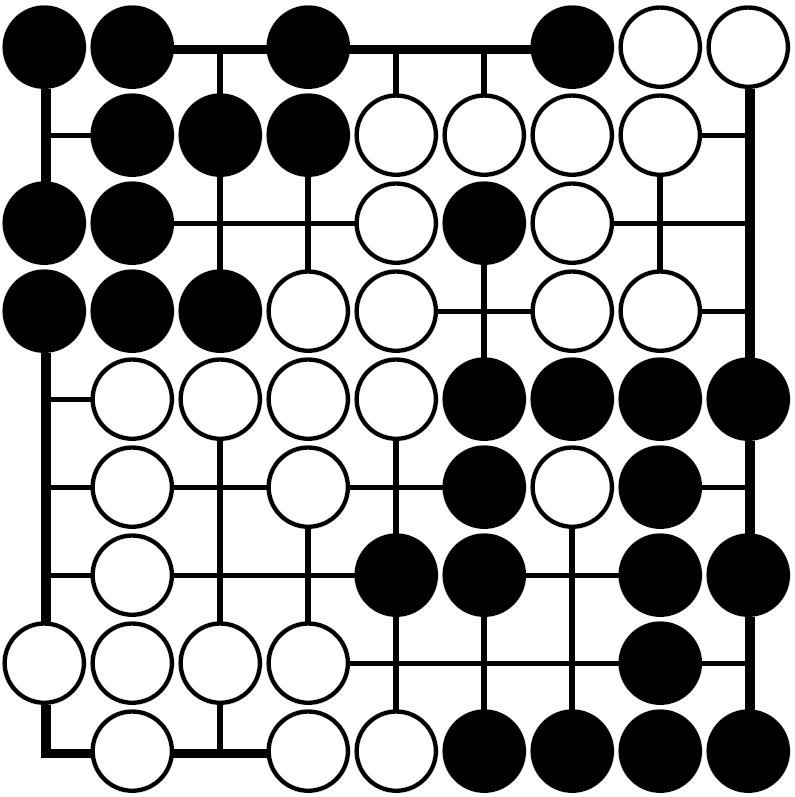
\includegraphics[width=.4\textwidth]{../img/late_endgame_Go_position_suited_for_exact_analysis.png}
    \captionWithCite{Late endgame position suited for exact analysis}{Muller1995computer}
    \label{fig:late-Go-endgame}
  \end{figure}

  Board partition improves when many safe walls are on~the board.
  In the opening and midgame, any partition can be approximate at best.
  In the endgame, the partition gets more precise when the status of~all big groups has been settled, and the outlines of~territories are clear.
  When stones become ``immortal'', significant parts of~the board definitely belong to one of the players.
  The connected components of~the rest of~the board form local games that are independent from each other.

  If each local game is simple enough to~analyze completely (such as in Figure~\ref{fig:late-Go-endgame}), combinatorial game theory can compute an~optimal move for the full board position.
\end{quotation}

\subsection{Playing Computer Go as a~Sum of~Local Games}

This is the general procedure for playing Go as a~sum of~local games used in~(\cite{Muller1995computer}):
\begin{enumerate}
  \item Board partition: find safe blocks, safe territories, and local areas.
  \item Generate local game trees in each area.
  \item Evaluate local terminal positions.
  \item Transform local game trees into mathematical games (and simplify games).
  \item Find an optimal move in the sum game and play it.
\end{enumerate}
\Mueller{} proposes heuristic algorithms for playing the entire game, and exact algorithms for late endgame positions.
Thus, the task of~solving endgames in 1995---at the age of Computer Go's infancy---already played a~vital role.

\subsection{A~Combinatorial Game Theory Framework for Approximate Play of~Sum Games}

\Mueller{} also suggests to replace the ``standard model'' of~computer Go by a~sum game model.
The following benefits and problems of~the sum game model for computer Go are listed in~(\cite{Muller1995computer}):

\medskip

\underline{Benefits}
\begin{itemize}[+]
  \item The model is well suited to the knowledge and style of~\textit{(at that time)} current Go programs:
    they concentrate on local fighting and surrounding territories.
  \item Locality reduces the complexity of~move generation and position evaluation.
    With the emphasis on~evaluation, clever pruning during move generation is not as crucial as in~global search because of~the reduced search space.
  \item Stepwise, directed expansion of~search is supported.
    This provides more time control than the usual iterative deepening.
    It is easy to use opponent's time.
  \item Important Go terms can be expressed or~refined in terms of~the theory, and need not be programmed separately.
  \item The reuse of~local game analysis improves efficiency while playing a~game.
  \item Parallelism emerges naturally on~many levels: local searches are independent, evaluation and operations on mathematical games can be parallelized.
\end{itemize}

\underline{Problems}
\begin{itemize}[-]
  \item Managing incrementally changing sets of~local graphs in place of a single position adds complexity.
  \item Accurate board partition and recognition of~dependencies is crucial.
  \item The usual problems of~selective search appear in complicated local games:
    missing crucial moves leads to wrong evaluation.
  \item Non-constant local games may be overlooked completely, such as insecure ``territories'' which can be destroyed from the inside.
  \item In this model there is no concept of~long-range full board plans.
    This is probably not a~big issue until programs reach amateur Dan or even professional level.%
    \footnote{For an~update on the current situation, see Section~\ref{sec:AlphaGo}.}
\end{itemize}

\subsection{A~Sum Game Model for the Entire Game of~Go}

Citing~(\cite{Muller1995computer}), there are several obstacles of~heuristic board partition (in the sum game model).

\begin{enumerate}[(a)]
  \item the impossibility of a~perfect, precise split:
    \begin{quotation} \noindent
      When applying a~local game model to the opening or~midgame, the biggest obstacle is the fact that the board cannot be partitioned into independent subgames.
      Few areas are completely surrounded, and surrounding stones are not yet invulnerable.
      We develop heuristics for board partition that split the imperfectly surrounded areas of~the opening and midgame.
    \end{quotation}

  \item the dependencies between the resulting subgames: 
    \begin{quotation} \noindent
      An~unavoidable side effect of~heuristic partition are dependencies between the resulting local games.
      Simple strategies for dealing with dependencies are pretending the games are independent, or re-searching a~bigger merged game.
    \end{quotation}
    See Section~\ref{ssec:dependencies-of-subgames} for more details.

  \item the difficulty (or almost infeasibility) of~exhaustive search in still quite large subgames:
    \begin{quotation} \noindent
      Even after heuristic partition, areas remain that are too big for an~exhaustive search by a~computer Go program, which must produce a~move in a~few seconds or minutes.
      In such big areas we use selective search.
      Tree growth is controlled by limiting the number of~moves generated, and by stopping the search before reaching a~terminal position.

      There are two levels of~search control:
      for the whole sum game, search time must be distributed between local games.
      For each local game, we must decide which nodes to expand and which expert modules to use for search and evaluation.
      A~post-processing stage handles detected dependencies between games.
    \end{quotation}
\end{enumerate}

Hence, the sum game model makes the best sense during the endgame part.
This general principle is as well applicable in poker:
we wait until the late stage of~the game, when it has greater impact to refine and re-solve the reached endgames.

\subsection{Dependencies Between Local Games}
\label{ssec:dependencies-of-subgames}

(\cite{Muller1995computer}) warns against the dangers of~subgame dependencies:

\begin{quotation} \noindent
  Dependencies between games occur when the areas of~local games overlap during area expansion, and when constraints of~one local game are related to~another game.
  The effect of~such dependencies differs widely:
  often it is so small that independence is a~useful approximation.
  In cases when a~move works as a~\emph{double threat} however, dependency analysis is crucial.
\end{quotation}

Strategies for dealing with dependencies are:
\begin{itemize}
  \item Ignore the dependency, treat games as independent
  \item Prove that the dependency does not affect the value of~the sum, or play of~the sum game
  \item Merge mutually dependent local games, then re-search the combined game, possibly using previously generated information on single games
  \item Analyze the interaction between local games, then use a~specialized theory to compute the joint game value
\end{itemize}

\subsection{Local Search and Evaluation in the Endgame}

Here is an overview of treating endgames in~(\cite{Muller1995computer}):
\begin{quotation} \noindent
  Following board partition, the algorithm for converting a Go endgame into a combinatorial game consists of generation of local game trees, scoring of local terminal positions, and evaluation of local games as mathematical games.
  Finally, a move in the resulting sum game must be selected, and identified with a move in the Go position.

  Safe territories and dame points are games that can be evaluated statically.
  Other local games are analyzed by local game tree search.
  Terminal positions are evaluated, and the values backed up in the tree, resulting in a mathematical game evaluation of each node.

  The result of search and analysis is a complete description of possible endgame plays that makes perfect play possible.
  We save the results of local analysis in a database of local positions.
  During play, each full board position corresponds one-to- one to a set of local positions, one from each local game.
  Positions and their values are retrieved from the database.

  The value of a full board position is the sum of local position values.
  A sum game evaluation algorithm selects a sufficiently good or optimal move.
  We also consider an algorithm with lower memory requirements, which stores only a subset of the positions of a local game in the database.
  In this case, if play reaches a position not stored in the database, we must re-search the corresponding local game.
\end{quotation}
In greater details, there are several points and aspects worth mentioning:
\begin{enumerate}[(a)]
  \item endgame area
    \begin{quotation} \noindent
      An~endgame area consists of~unsettled stones, and of~empty points not yet surrounded by~either color.
      Safe stones, usually of~both colors, surround the area.
      During endgame play, unsettled stones either become safe or are captured.
      Empty points will become occupied, safe territory or dame.
      A~rare case are ``untouchable'' empty points in \emph{seki}.

      \begin{figure}[H]
        \centering
        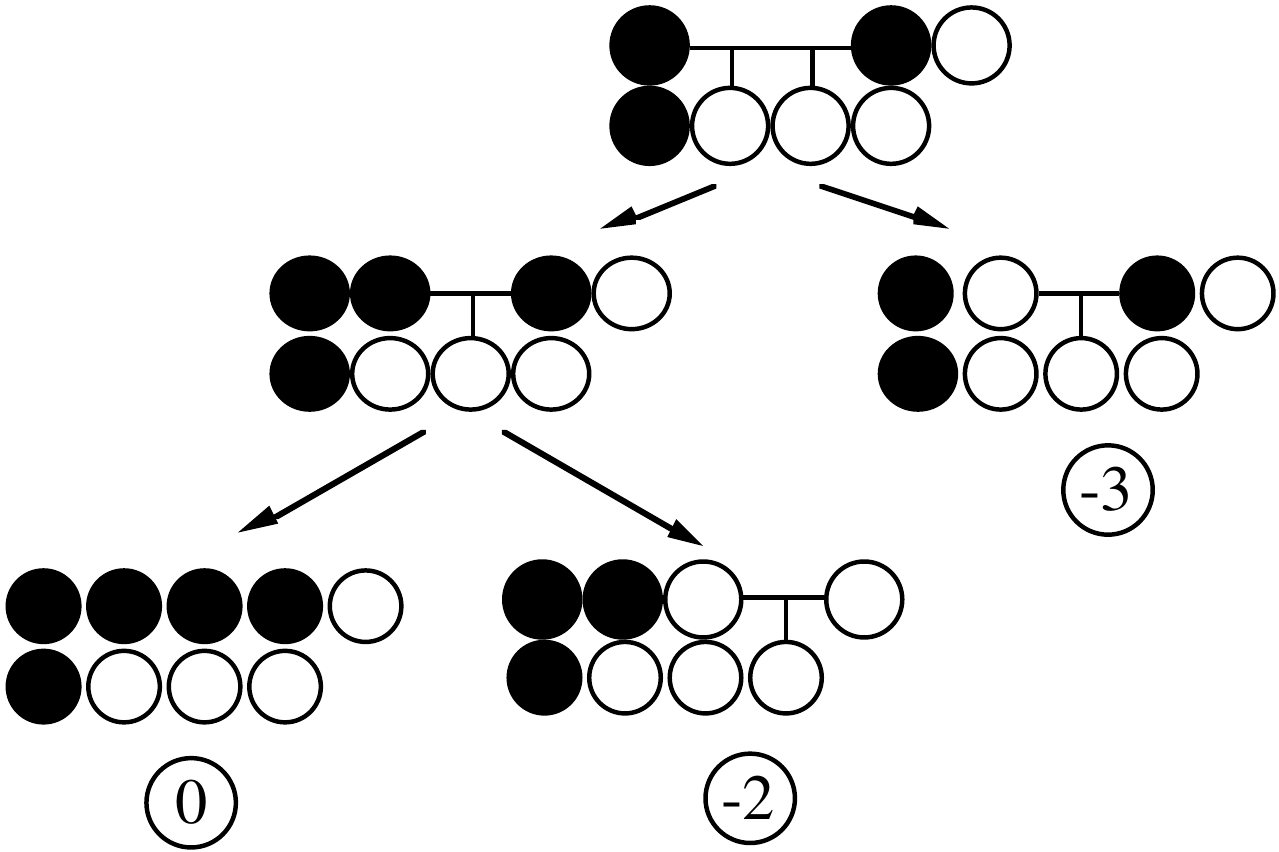
\includegraphics[width=.7\textwidth]{../img/Go_search_tree.png}
        \captionWithCite{Local game tree with evaluation of terminal nodes}{Muller1995computer}
      \end{figure}
    \end{quotation}

  \item move generation
    \begin{quotation} \noindent
      We generate all legal moves for both colors, except in a~terminal position or if moves can be pruned.
      Examples of~\emph{pruning rules} are restricting the number of~\emph{dame} moves generated to at most one, and pruning moves dominated by other moves.%
      \footnote{Compare with \emph{policy networks} of~AlphaGo in Section~\ref{sec:AlphaGo}.}
      \emph{Termination rules} decide when a~position can be evaluated statically, without further expanding the tree.%
      \footnote{Compare with \emph{value network} of~AlphaGo in Section~\ref{sec:AlphaGo}.}
    \end{quotation}

  \item terminal positions
    \begin{quotation} \noindent
      \noindent
      We recognize the following terminal positions:
      \begin{enumerate}[$\diamondsuit$]
        \item No legal moves
        \item No good move (all points are territory, or dame)
        \item Value of position known from transposition table, pattern, or local position database
      \end{enumerate}
      The first two types of~terminal positions evaluate to a~number, or number-plus-star (odd
      number of~dame).
      If the value of a~position is known from another source, it is terminal in the sense that there is no need to continue search.
      The value itself can be any mathematical game value.
      Non-terminal positions may have a~constant value as well, if the outcome is the same no matter who plays first, but this has to be proven using search.
    \end{quotation}

  \item scoring
    \begin{quotation} \noindent
      Scoring assigns a~number, or number plus dame, to a~terminal position.
      In Chinese rules, scoring measures how many stones and empty points belong to either color.
      In Japanese rules, territory and prisoners are counted.
      Both kinds of~scoring are straightforward in the endgame because safe and dead stones, territories and neutral points are known exactly.%
      \footnote{See Section~\ref{sec:Go}.}
    \end{quotation}

  \item exact play on a~subset of~the board
    \begin{quotation} \noindent
      When board partition indicates that big areas remain, or search cannot solve all small areas, the user interface offers three options:
      \begin{enumerate}[$\diamondsuit$]
        \item Stop playing
        \item Ignore the unsolvable big areas
        \item Use heuristic play in the big areas
      \end{enumerate}
      Even if an original position has been solved, suicidal opponents can cause problems later:
      they might endanger their ``immortal'' stones, which violates our initial assumptions on board partition and generates new unstable positions where optimal play might be very complicated.
    \end{quotation}

  \item saving results of~local search
    \begin{quotation} \noindent
      Positions encountered during local search are stored in \emph{a~database of~local games}.
      An~important question is what to store:
      There is a~tradeoff between recomputation time and required storage.
      For building a~permanent database, it makes sense to store only ``difficult'' moves in the database, and recalculate the rest if needed.
      It is efficient to store which moves are locally good or bad, but omit refutations:
      the trees proving that bad moves are inferior.
      Such a~database is sufficient for playing against a~good opponent.
      Only in the unlikely case of~locally bad opponent play, we must recalculate one subtree to find a~refutation.
      The Table~\ref{tab:db-loc-games} lists some possibilities.
    \end{quotation}
    \begin{table}[!htbp]
      \centering
      \begin{tabular}{ |p{.45\textwidth}|p{.48\textwidth}| } 
        \hline
        \textbf{Type of database} & \textbf{Content} \\
        \hline
        Full                            & All positions encountered during exhaustive search \\
        Color-complete (Black or White) & All positions reachable by non-dominated moves of~color and arbitrary opponent moves (pruned bad moves of~color) \\
        Optimal                         & At least one position corresponding to each non-dominated option of each reachable position, guarantees optimal play from each position in~database \\
        Ko-complete (Ko-optimal)        & Complete (optimal) + possible Ko threats and answers \\
        Sufficiently good               & Guarantees optimal score from a~starting position, might fail to exploit some opponent mistakes \\
        \hline
      \end{tabular}
      \caption{Possible database variants of~local games}
      \label{tab:db-loc-games}
    \end{table}

  \item pruning game trees 
    \begin{quotation} \noindent
      The evaluation of~nodes leads to pruning the game tree:
      moves to dominated options are marked as locally bad moves.
      With the usual domination test for $\geq$, all but the first of~several equally good moves are pruned.
      A~test for $>$ keeps the full set of~equally good moves.
    \end{quotation}

  \item mapping a~move in the abstract game to a~Go move
    \begin{quotation} \noindent
      As a~last step, we must find a~Go move corresponding to the selected option in the abstract game.
      We select the first move with sufficient \emph{incentive}.
    \end{quotation}
\end{enumerate}

\subsection{Speeding up Local Search}

(\cite{Muller1995computer}) considers various improvements to computational efficiency:
\begin{quotation} \noindent
  Ignoring illegal moves and captures, the number of possible plays in an $n$ point area is approximately $2n$ ($n$ for each player), and play generates a $n-1$ point area.
  A~rough estimate for the size of~the game tree is therefore $2n\cdot2(n-1)\cdot \ldots \cdot2 = 2^n n!$

  Due to this combinatorial explosion, even fairly small endgames become prohibitively expensive to compute using this approach.
  In the following, we look at a~number of~techniques for reducing the size of the search tree.
\end{quotation}

\begin{enumerate}[(a)]
  \item transposition table (see also Table~\ref{tab:reduction-transp-tab})
    \begin{quotation} \noindent
      A~transposition table detects identical board positions, reducing the size of~the search space from $\approx 2^n n!$ to $3^n$ states.

      \begin{table}[!htbp]
        \centering
        \begin{tabular}{ |rrr| }
          \hline
          \textbf{$n$} & \textbf{$2^nn!$} & \textbf{$3^n$} \\
          \hline
          1	&	2	&	3 \\ 
          2	&	8	&	9 \\ 
          3	&	48	&	27 \\ 
          4	&	384	&	81 \\ 
          5	&	3840	&	243 \\ 
          6	&	46080	&	729 \\ 
          7	&	645120	&	2187 \\ 
          8	&	10321920	&	6561 \\ 
          9	&	185794560	&	19683 \\ 
          10	&	3715891200	&	59049 \\ 
          \hline
        \end{tabular}
        \caption{Reduction of search space by transposition table}
        \label{tab:reduction-transp-tab}
      \end{table}
    \end{quotation}

  \item pruning moves
    \begin{quotation} \noindent
      The width of~the search tree can be further reduced by pruning moves.
      In contrast to selective search, we may only eliminate moves that are provably worse-or-equal than others.
      If a~move achieves all points of~the local area, or if any other move would give the opponent an~answer which achieves the maximum score, the move is optimal, and we can prune all other moves.
    \end{quotation}
\end{enumerate}

\subsection{Using Combinatorial Game Theory to Solve Late Endgames by Computer}

These are some objectives that can be accomplished by the approach of~(\cite{Muller1995computer}):
\begin{itemize}
  \item Perfect computer play in late endgame
  \item Find the game-theoretic value of a position long before the end
  \item Evaluate the opponent’s endgame moves
  \item Find moves that are good enough even with a reduced local game database
\end{itemize}
On the other hand, the work also remarks that strict analysis of~endgames is not possible with this method if one of the following limits is reached:
\begin{itemize}
  \item \textbf{Partition:}
    too few blocks can be proven safe independent of~endgame play.
    Therefore some areas become too big for complete search.
  \item \textbf{Summation:}
    no move with dominating incentive exists, and both summing and partial search take too long.
  \item \textbf{Ko:}
    Standard combinatorial game theory exploits the independence of~local games.
    In the case of~Ko, the independence is broken (a~locally bad move may be globally best if it serves as a~Ko threat).
    Generalizations of~the theory to handle Kos are a topic of [at that time] current research.
  \item \textbf{Added complexity in ‘obvious’ situations:}
    In cases where the focus of~play is obvious (i.e. only one local situation is relevant), combinatorial game theory introduces additional complexity by investigating moves for both players in this and each other position.
\end{itemize}

\subsection{Time and Memory Management}

One reason why endgames are exhaustively studied is due to their computational benefits.
As the game progresses, more exact analysis can be done, and thus, time and memory resources may be better utilized.
In particular, (\cite{Muller1995computer}) uses following ``adaptive'' resource adjustments:

\begin{enumerate}[(a)]
  \item memory management of objects and local trees
    \begin{quotation} \noindent
      In a~program with limited memory, we need to decide which local game nodes and other calculated results to keep, and which to dispose during the course of play.
      Which items are obsolete, and which can probably be reused later?
      Only heuristic rules for memory management are possible, because the future actions of~the user are unpredictable.

      During the course of a~game there is a~gradual shift of~relevance.
      Starting a~new game leads to radical change, just about all computed results are useless in the new game.
      Some flexibility for users undoing moves should be provided.

      As a~solution we define a~\emph{forced substate}, a subset of all points on the current board.
      The substate consists mainly of~safe-looking stones.
      We delete all objects that do not match the forced substate.
      For supporting undo’s, we exclude all points affected by the last two moves from the points of~the forced substate.
      Some items are exempt from automatic disposal:
      user inputs, and objects explicitly calculated on a~user’s demand.
    \end{quotation}

    \parbox{.9\textwidth}{
    \item time control for tournament play
      \begin{quotation} \noindent
        Time control determines how much time to use for each subgame, for tactics, and for
        Life\&Death problems. [$\dots$]
        The same algorithm with smaller time slices could be used for computing in opponents time.
        A~fast mode is used in time trouble:
        only minimal time is used for subproblems such as tactics calculations and Life\&Death.
      \end{quotation}
    }

\end{enumerate}

\subsection{Pattern Learning}

Pattern recognition is one of~the key components of~AlphaGo (see Section~\ref{sec:AlphaGo}).
Arguably, the program's success might be partially attributed to learning Go patterns from human expert plays.
For comparison, (\cite{Muller1995computer}) reports the following state of~``Go-related Research in Visual Perception, Machine Learning and Neural Networks'' in 1995:
\begin{quotation} \noindent
  Go has been used as a~vehicle for research in~visual perception, machine learning and neural networks (\cite{Wilcox79}, \cite{Enderton1991golem}, \cite{Stoutamire1991machine}, \cite{Schraudolph1994temporal}).
  Starting from only the rules of~the game, learning programs can typically pick up basic Go principles, such as saving a~stone from capture, or making a~[one-point] jump.

  A~most disturbing fact is that since Wilcox’ pioneering efforts, none of~this research has been applied to a~state-of-the-art Go program.
  The problems of~automatically tuning and expanding an~existing knowledge base, or learning of~new high-level concepts, seem quite different from the ab-initio learning problems that have been researched.

  Low level concepts can be learned, but they have already been programmed in the better programs.
  Neural networks can be trained to play locally good shapes, but have no clue when to play it.%
  \footnote{This assertion, in particular, has changed with AlphaGo.}
  Such programs fall easy prey to those that know more about tactics and Life\&Death.
\end{quotation}
(\cite{Muller1995computer}) also suggests pattern matching as a~promising mean for improvement:
\begin{quotation} \noindent
  Research on pattern learning in computer Go has unfortunately been restricted to \emph{ab-initio} learning of~the most basic patterns from zero knowledge.
  Interactive or automatic tuning and expansion of a~state-of-the-art pattern base is another fascinating research topic.
\end{quotation}

\subsection{Contributions of~Combinatorial Game Theory to Go Endgames}

The doctoral thesis (\cite{Muller1995computer}) highlights following contributions to general computer science:
\begin{itemize}
  \item Scientists are fascinated by problems which can be stated simply, yet are hard to solve.
    Computer Go is a~prime example.
    We have brought the divide-and-conquer approach, a~fundamental paradigm of~computer science, to bear on computer Go.

  \item The application of a~sophisticated mathematical theory to computer Go provides an~example of~algorithms for a~nontrivial decomposition of a~complex problem.
\end{itemize}
Another contributions are the ones aiding computer Go endgames specifically:
\begin{itemize}
  \item We have implemented a~\emph{late endgame player}, a~niche where program play surpasses human play in both speed and exactness.
    We did this by applying concepts from combinatorial game theory to Go.
    The program plays a~wide variety of`late endgame positions perfectly.

  \item We have developed algorithms for board partition and dependency analysis.
    The central idea of~board partition has been used both in a~program following a~traditional model, and in a~program based on the sum game approach.
\end{itemize}
Hence, the work employs a~technique of~applying an~elaborate mathematical theory (of~combinatorial game theory) to deal with the endgame phase.
In particular, CGT is used to ``connect'' individual relevant subgames, which may be solved independently.

As we will see later, the situation in the case of~Poker is slightly more delicate:
the imperfect-information property prevents us from using an~immediate divide-and-conquer approach.
Instead, we will \emph{augment} the information by saturating it with additional game states (see Section~\todo).

\note{
  \label{note:CGTvsAlphaGo}
  It is also interesting to compare the method of~(\cite{Muller1995computer}) with the modern approach of~\emph{AlphaGo}:
  the ad-hoc Go-specific knowledge is replaced with general-learning neural networks and the probabilistic \emph{Monte Carlo Tree Search} algorithm.
  Such a~combination has the capability to surpass professional human players at the highest ranks.
  On top of that, this solution can be adapted to other games without substantial modifications.
  As long as there is an~abundance of~available data, the system can always be trained with no need to imbue it with any game-specific knowledge.
  See Section~\ref{sec:AlphaGo} for more details.
}

\section{Go Endgames Using Artificial Intelligence}
\label{sec:AlphaGo}

As of~today, over 20 years have passed since \Mueller's work.
\emph{DeepMind}, a~London-based AI start-up recently acquired by Google, has developed the strongest computer Go program so far:
\emph{AlphaGo}.

This section is based on~the article ``Mastering the game of Go with deep neural networks and tree search''~(\cite{Silver2016mastering}), which documents the internals of~AlphaGo:

\begin{quotation} \noindent
  The game of~Go has long been viewed as~the most challenging of~classic games for artificial intelligence owing to its enormous search space and the difficulty of~evaluating board positions and moves.

  Here we introduce a~new approach to computer Go that uses \emph{value networks} to evaluate board positions and \emph{policy networks} to select moves.
  These deep neural networks are trained by a novel combination of supervised learning from human expert games, and reinforcement learning from games of self-play.
  Without any lookahead search, the neural networks play Go at the level of~state-of-the-art Monte Carlo tree search programs that simulate thousands of~random games of~self-play. 

  We also introduce a~new search algorithm that combines Monte Carlo simulation with value and policy networks.
  Using this search algorithm, our program AlphaGo achieved a~99.8~\% winning rate against other Go programs, and defeated the human European Go champion by 5 games to~0.
  This is the first time that a~computer program has defeated a~human professional player in the full-sized game of~Go, a~feat previously thought to be at least a~decade away.
\end{quotation}
For more details, also consult my presentations on AlphaGo given at:
\begin{itemize}
  \item Spring School of Combinatorics 2016 (Charles University in Prague): \\
    \href{http://www.slideshare.net/KarelHa1/mastering-the-game-of-go-with-deep-neural-networks-and-tree-search-presentation}
    {\tt http://www.slideshare.net/KarelHa1/mastering-the-game-of-go\\-with-deep-neural-networks-and-tree-search-presentation}

  \item Optimization Seminar (Charles University in Prague) \\
    \href{http://www.slideshare.net/KarelHa1/alphago-mastering-the-game-of-go-with-deep-neural-networks-and-tree-search}
    {\tt http://www.slideshare.net/KarelHa1/alphago-mastering-the-game\\-of-go-with-deep-neural-networks-and-tree-search}

  \item Distributed Computing group (ETH \Zurich) \\
    \href{http://www.slideshare.net/KarelHa1/alphago-for-disco-group-of-eth-zurich}
    {\tt http://www.slideshare.net/KarelHa1/alphago-for-disco-group\\-of-eth-zurich}
\end{itemize}

\subsection{Game-Tree Search}

Optimal value~$v^*(s)$ determines the~outcome of~the game from every board position $s$ under perfect play by~all players.
This value can be computed by~recursively traversing the~search tree containing approximately $b^d$ possible sequences of moves, where $b$ is the breadth of~game (number of legal moves per position) and $d$ is its depth (game length).

In~the case of~chess, that is $b \approx 35$ and $d \approx 80$, whereas Go has $b \approx 250$ and $d \approx 150$.
This amounts to a~terrifying overnumerousness: there are more Go positions than atoms in the observable Universe.
Furthermore, ``that makes Go a~googol [$10^{100}$] times more complex than chess'',%
\footnote{\href{https://deepmind.com/alpha-go.html}{https://deepmind.com/alpha-go.html}}
and therefore, exhaustive search is deemed intractable.

How to handle the size~of the game tree? For the$\dots$
\begin{itemize}
  \item $\dots$breadth: we train a~neural network to~select moves.
  \item $\dots$depth: we train a~neural network to~evaluate the current position.
  \item $\dots$tree traverse: we use Monte Carlo tree search method.
\end{itemize}

\textbf{Monte Carlo tree search} (MCTS) is a~Monte Carlo heuristic of~the classical tree search.
However, instead of traversing the entire game tree, the MCTS selects the~most promising moves, expanding the search tree based on~random sampling.

In~each iteration, the game is played-out to~the very end by~choosing moves at~random.
The final outcome of~each playout is then used to~weight the nodes in~the game tree accordingly.
Thus, better nodes are more likely to be chosen in future playouts.

\begin{figure}[H]
  \centering
  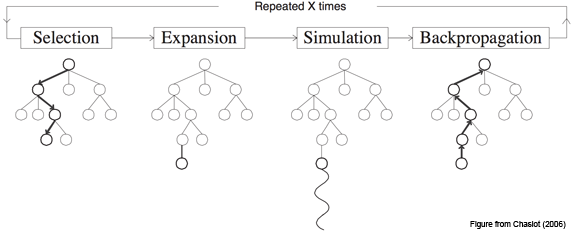
\includegraphics[width=.6\textwidth]{../img/MCTS.png}
  \caption{The scheme of~MCTS}
  \label{fig:MCTS}
\end{figure}

\subsection{Neural networks}

Inspired by biological neural networks, an~artificial neural network (ANN) is a~network of~interconnected nodes that make up a~model.
ANNs can be defined as~statistical learning models that are used to approximate functions which depend on a~large number of~inputs.
Neural networks are typically used when the volume of~inputs is far too large for~standard machine learning approaches.

\begin{figure}[H]
  \centering
  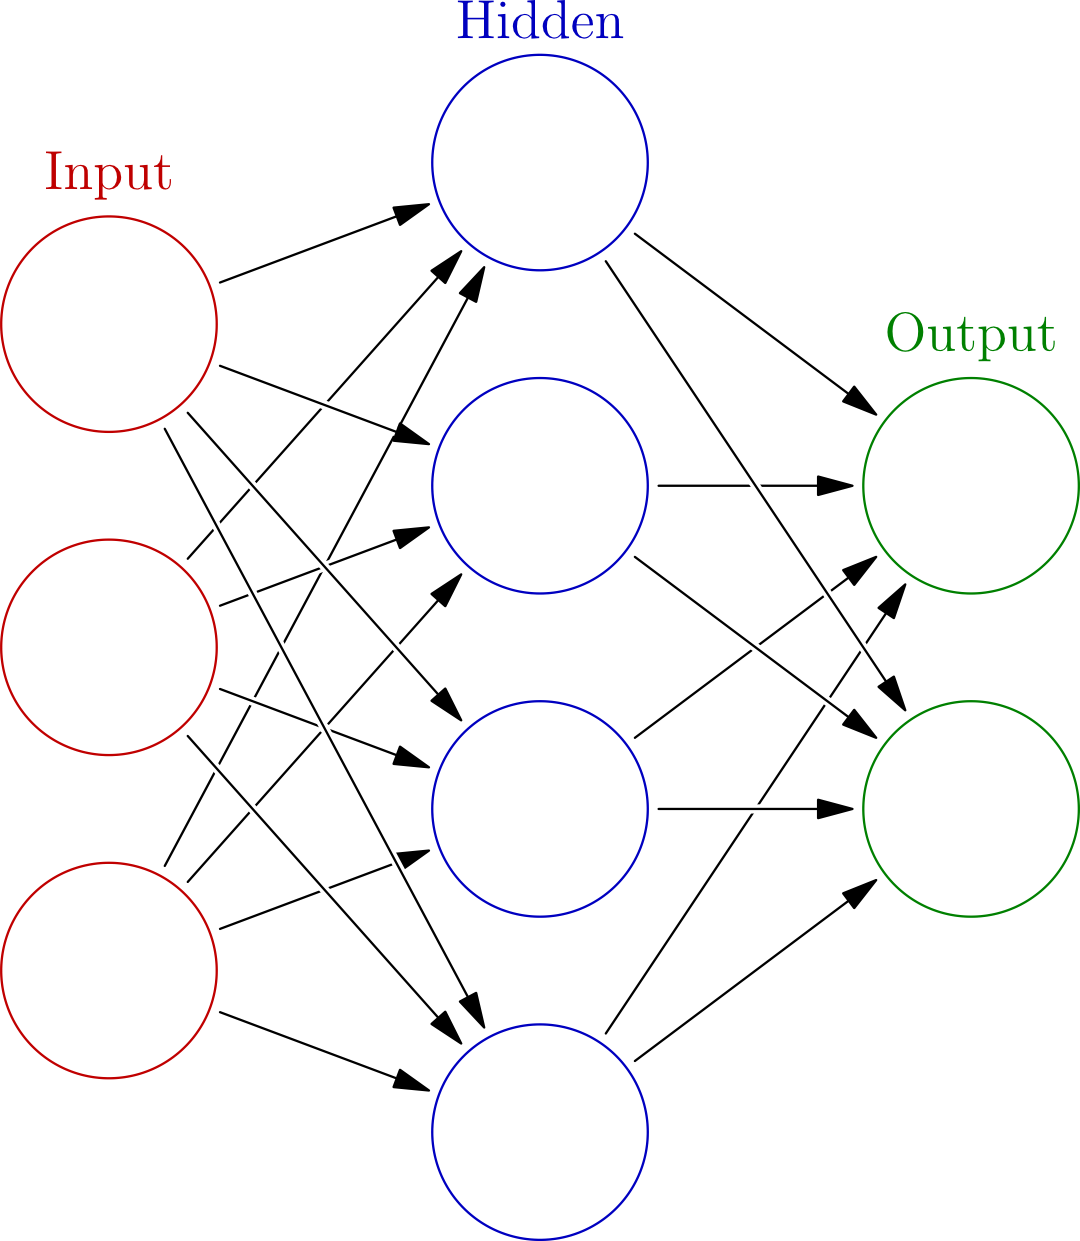
\includegraphics[height=.2\textheight]{../img/colored_neural_network.png}
  \caption{A~shallow neural network with 3 layers}
  \label{fig:shallow-neural-network}
\end{figure}

\textbf{Convolutional neural network} (CNN) is a~neural network suitable for high-dimensional inputs (e.g. a~large number of~pixels in an~image).
CNNs are frequently used in~computer vision (for identifying objects in an~image, for face detection in~photos etc.).
They are invariant to expectable transformations of~input, such as translations of~objects in~a~picture or changes in~illumination.

\textbf{Deep neural network} (DNN) is a~neural network with many hidden layers.
It can model complex non-linear relationships, e.g. in~speech, in~images, in~videos or in~board positions of~Go.

\subsection{Pipeline of Neural Networks}

AlphaGo employs two kinds of deep convolutional neural networks---a~\emph{policy network} (for move selection) and a~\emph{value network} (for board evaluation).
\begin{figure}[H]
  \centering
  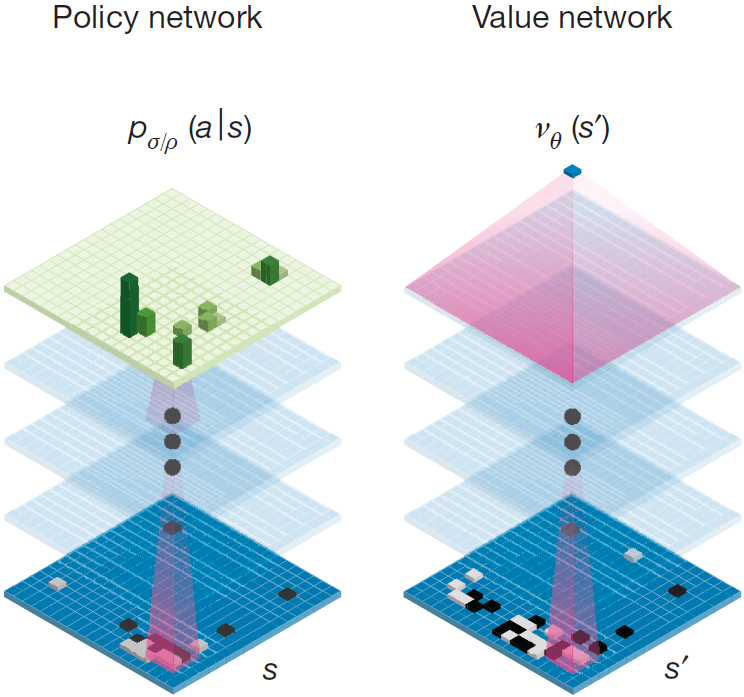
\includegraphics[width=.5\textwidth]{../img/policy_and_value_network.png}
  \captionWithCite{Comparison between policy and value network}{Silver2016mastering}
  \label{fig:policy_vs_value_nets}
\end{figure}

In the following Figure~\ref{fig:neural_nets_pipeline}, we can view the whole training process of~AlphaGo's neural networks.
\begin{figure}[H]
  \centering
  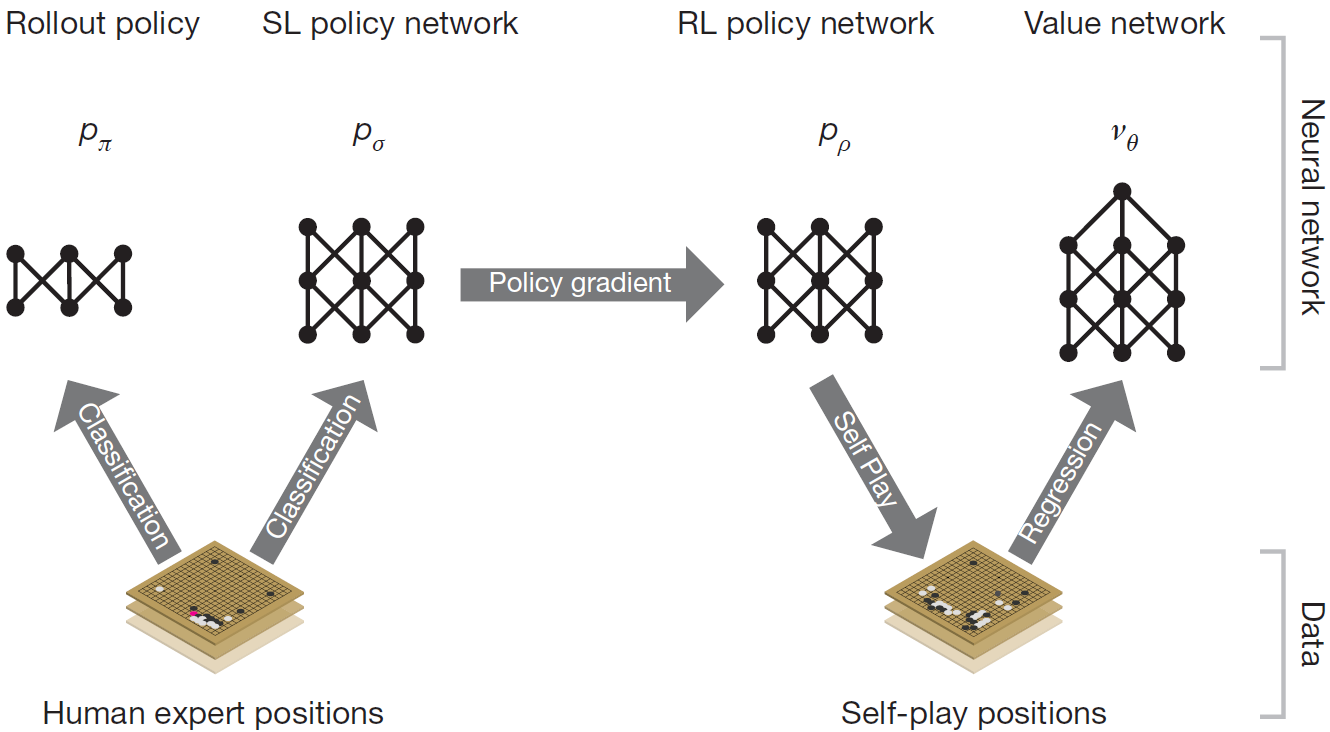
\includegraphics[width=.7\textwidth]{../img/neural_nets_pipeline.png}
  \captionWithCite{Training the neural networks of~AlphaGo: the~pipeline~and~the~architecture}{Silver2016mastering}
  \label{fig:neural_nets_pipeline}
\end{figure}

\textbf{Rollout policy} $p_\pi$ is a~CNN rapidly sampling actions during a~\emph{rollout} (a~fast-forward simulation from a~position to the end of~the game).
It predicts expert human moves much faster but less accurately than $p_\sigma$ (see below).
The output is a~probability distribution over all moves.

\textbf{Policy network} is a~CNN selecting moves.
It addresses the problem of the game-tree breadth.
There are two flavors of~these networks:
\begin{itemize}
  \item \textbf{SL policy network} $p_\sigma$ is trained by \underline{s}upervised \underline{l}earning to predict expert human moves.
  \item \textbf{RL policy network} $p_\rho$ is trained by \underline{r}einforcement \underline{l}earning to win in the~games of~self-play.
\end{itemize}

\textbf{Value network} $v_\theta$ is a~CNN evaluating board positions, so as to address the problem of the game-tree depth.
It is trained by regression to predict the outcome in~positions of~the self-played games.

\subsection{Main Algorithm}

Finally, the neural networks are combined with MCTS into the main algorithm.

During the play, AlphaGo simulates up to 100 possible continuations per each move by selecting the most promising actions and following them.
This way, it descends the game-tree down to a~depth given by a~parameter.
At that point, leaf nodes are evaluated in two ways:
\begin{enumerate}[(1)]
  \item using the dedicated value network $v_\theta$,
  \item simulating the self-play until the terminal positions, using the fast rollout policy $p_\pi$.
\end{enumerate}
The two are mixed into the final value of~the leaf node.

Once every simulation of a~single round is finished, all new values are backpropagated to the root, thus updating necessary variables on the way up.

For more details, consult (\cite{Silver2016mastering}) or the before-mentioned presentations.

\note{
  Main algorithm demonstrates the connection to \emph{our theme of~endgames}:
  the simulations may be viewed as ``solving endgames''.
  In particular, the $p_\pi$ rollouts somehow remind of~exhaustive search for the game value during the late stage of~the play.
  In this sense, the approaches of~AlphaGo and endgame computation bear a~striking similarity.

  On the other hand, AlphaGo performs the same simulation algorithm during the whole game:
  from an~empty board until the final move.
  Therefore, it would be imprecise to talk about ``endgame'' here.
}

\subsection{Playing Strength}

In order to assess the playing strength of~AlphaGo, DeepMind has organized an~internal tournament between different other Go programs,%
\footnote{\emph{CrazyStone} and \emph{Zen} are the strongest commercial programs, whereas \emph{Pachi} and \emph{Fuego} are strongest among the open-source ones.}
as well as a~duel of~AlphaGo against the European Go Champion Fan Hui.
Figure~\ref{fig:Go-tournament} displays the outcome of the tournament:

\begin{quotation} \noindent
  Each program used approximately 5 s computation time per move.
  To provide a~greater challenge to AlphaGo, some programs (pale upper bars) were given four handicap stones (that is, free moves at~the start of~every game) against all opponents.
  Programs were evaluated on an Elo scale: a~230 point gap corresponds to a~79\% probability of winning, which roughly corresponds to one amateur dan rank advantage on KGS;
  an~approximate correspondence to human ranks is also shown, horizontal lines show KGS ranks achieved online by that program.
  Games against the human European champion Fan Hui were also included;
  these games used longer time controls.
  95\% confidence intervals are shown.~(\cite{Silver2016mastering})
\end{quotation}

\begin{figure}[H]
  \centering
  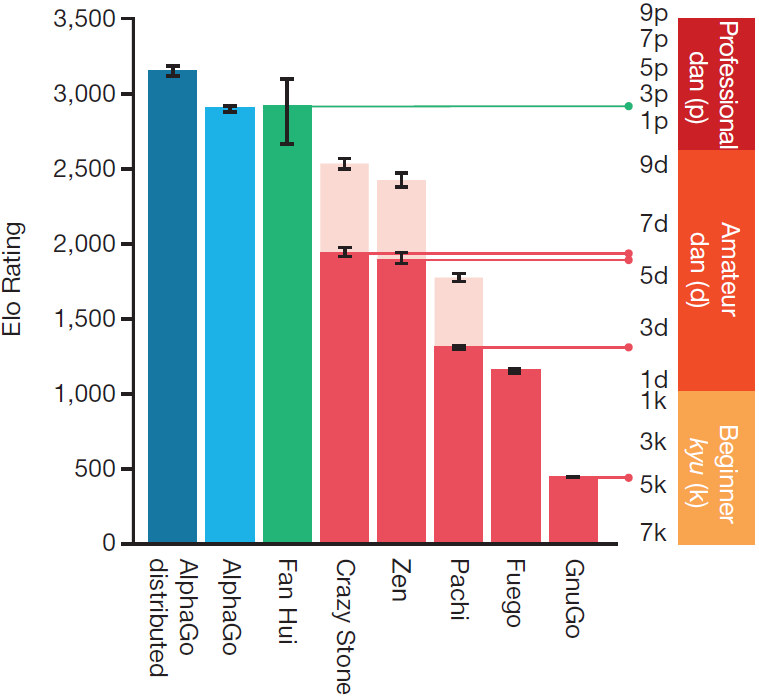
\includegraphics[width=.5\textwidth]{../img/results_of_tournament.png}
  \captionWithCite{Tournament with other programs and Fan Hui}{Silver2016mastering}
  \label{fig:Go-tournament}
\end{figure}

Here is an~official report provided by Google DeepMind%
\footnote{\href{https://deepmind.com/alpha-go.html}{https://deepmind.com/alpha-go.html}}
about AlphaGo's matches against human professionals:
\begin{quotation} \noindent
  After our program AlphaGo won 5--0 in a~formal match on~October 2015, against the reigning 3-times European Champion, Fan Hui, becoming the first program to ever beat a~professional Go player in an~even game;
  AlphaGo then went on to complete its ultimate challenge.

  In March 2016 AlphaGo won 4--1 against the legendary Lee Sedol, the top Go player in the world over the past decade.
  The matches were held at the Four Seasons Hotel, Seoul, South Korea on March 9\textsuperscript{th}, 10\textsuperscript{th}, 12\textsuperscript{th}, 13\textsuperscript{th} and 15\textsuperscript{th} and livestreamed on DeepMind’s YouTube channel as well as broadcast on TV throughout Asia through Korea’s Baduk TV, as well as in China, Japan, and elsewhere.

  They were played under Chinese rules with a~komi of~$7.5$ (the compensation points the player who goes second receives at~the end of~the match).
  Each player received two hours per match with three lots of 60-second byoyomi (countdown periods after they have finished their allotted time).
\end{quotation}

Following from this, computers seem to have reached the ``superhuman'' level of~expertise and they now appear to be superior to humans in~the game of~Go.
